\section{Experiment 1 : Getting Started}
\subsection{Running Wireshark}
    \subsubsection*{Problems}
    \begin{enumerate}[label=\bfseries Problem \arabic*:,leftmargin=*,labelindent=1em]
        \item List 3 different protocols that appear in the protocol column in the unfiltered packet-listing window in step 7 above.\\[0.2mm]
            % 답을 \soln 뒤에 작성하면 됨 
            \soln TCP, DNS, TLSV ... etc
        \item How long did it take from when the HTTP GET message was sent until the HTTP OK reply was received? 
        (By default, the value of the Time column in the packet-listing window is the amount of time, in seconds, 
        since Wireshark tracing began. To display the Time field in time-of-day format,
        select the Wireshark View pull down menu, then select Time Display Format, then select Time-of-day.) \\[0.2mm]
            \soln It tooks 0.002608 (sec)
            \vspace{-4mm}  
            \begin{figure}[!h]\centering
            \hspace{15mm} 
        		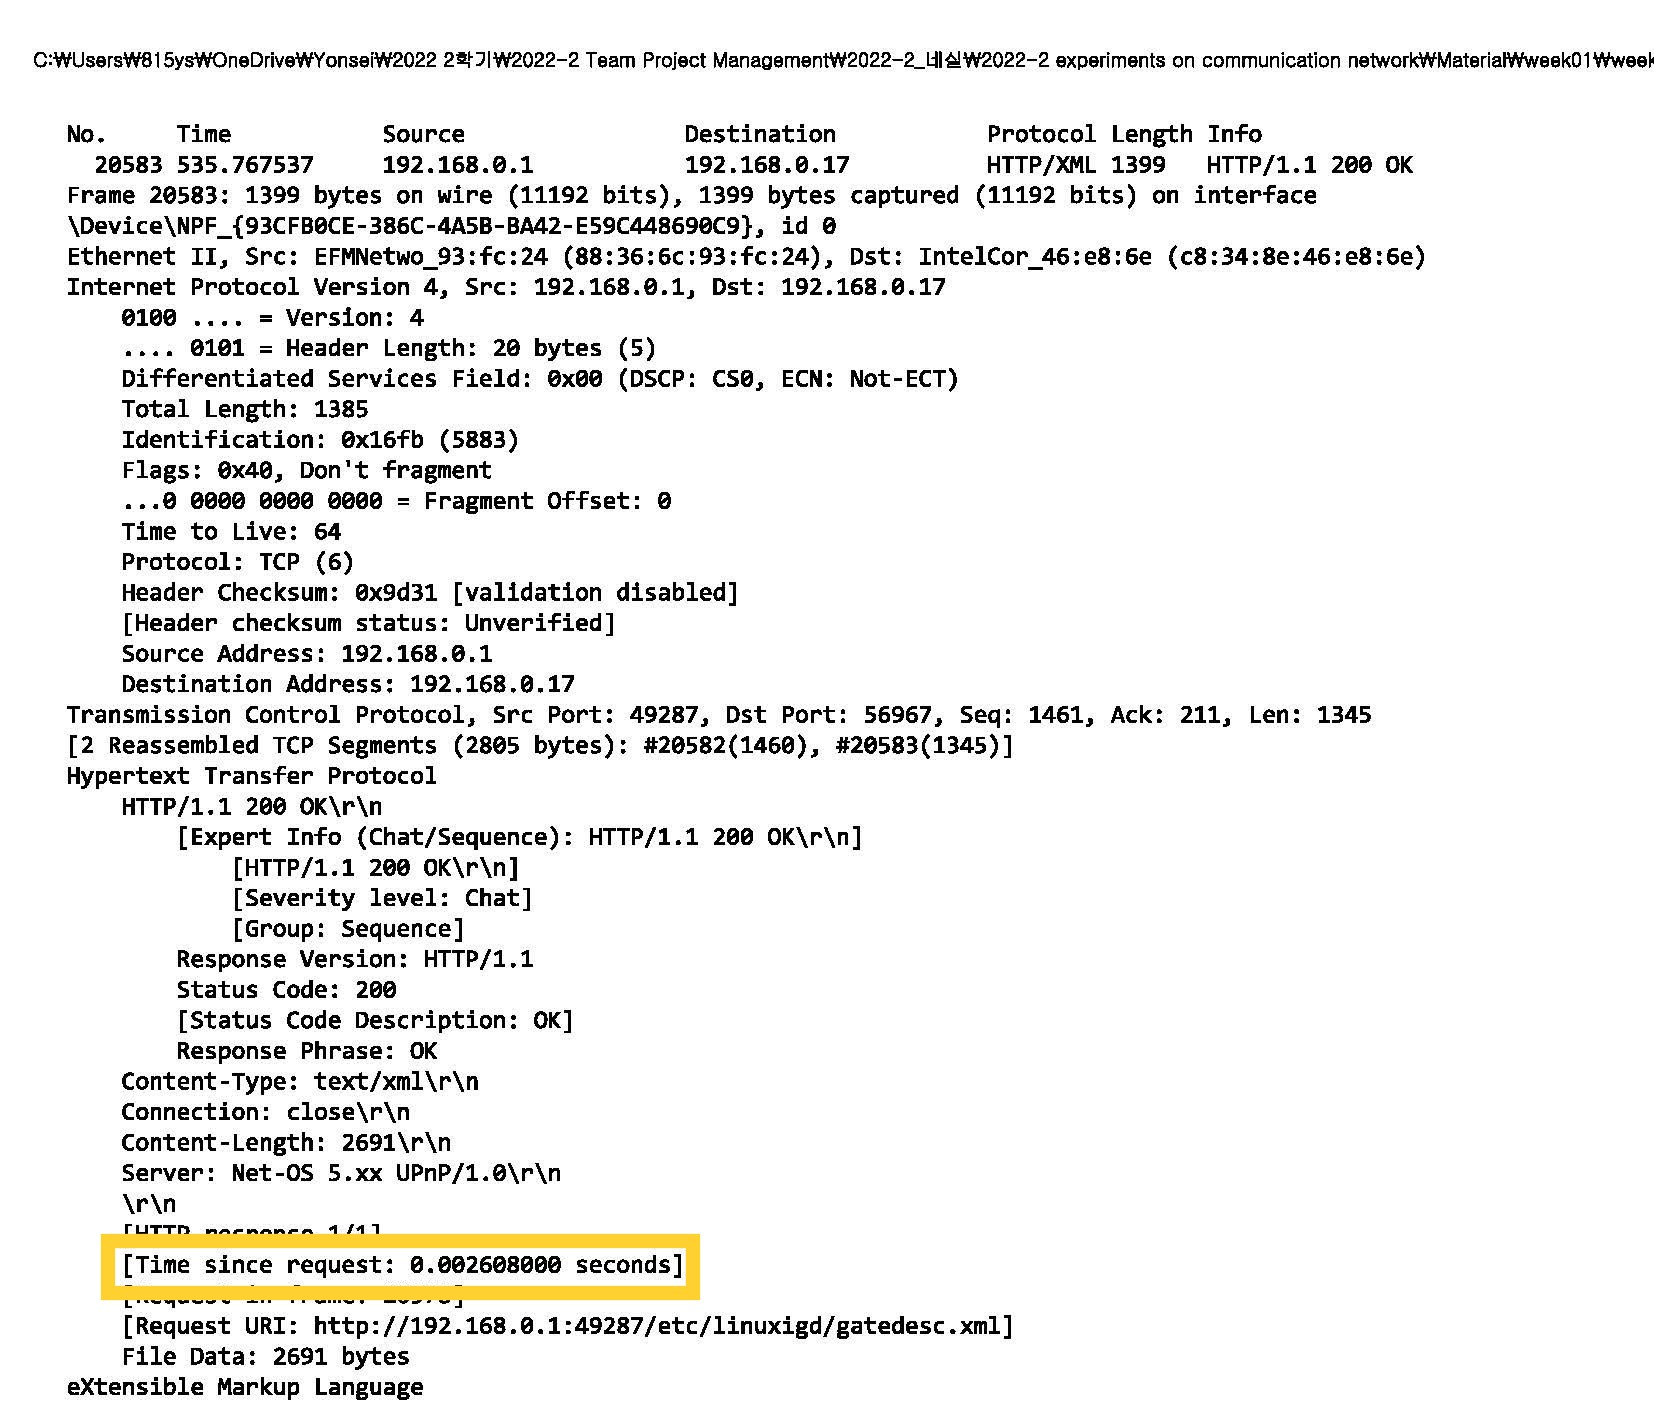
\includegraphics[width=.85\textwidth]{image/result_week01/Q1-2.jpg}
        		\caption{\footnotesize Problem 1-2's screenshot : Packet-HTTP/1.1 200 OK}
        		\vspace{-10pt}
            \end{figure}
        \item What is the Internet address of the gaia.cs.umass.edu (also known as wwwnet.cs.umass.edu)? 
        What is the Internet address of your computer?\\[0.2mm]
            \soln Since the packet I print out is the replied message from gaia.cs.umass.edu.
            The source adr that value of 192.168.0.1 is the gaia.cs.umass.edu ‘s adr, and the destination adr, 192.168.0.17 is the internet adr of my computer.
\newpage
            \vspace{-4mm}  
            \begin{figure}[!h]\centering
        		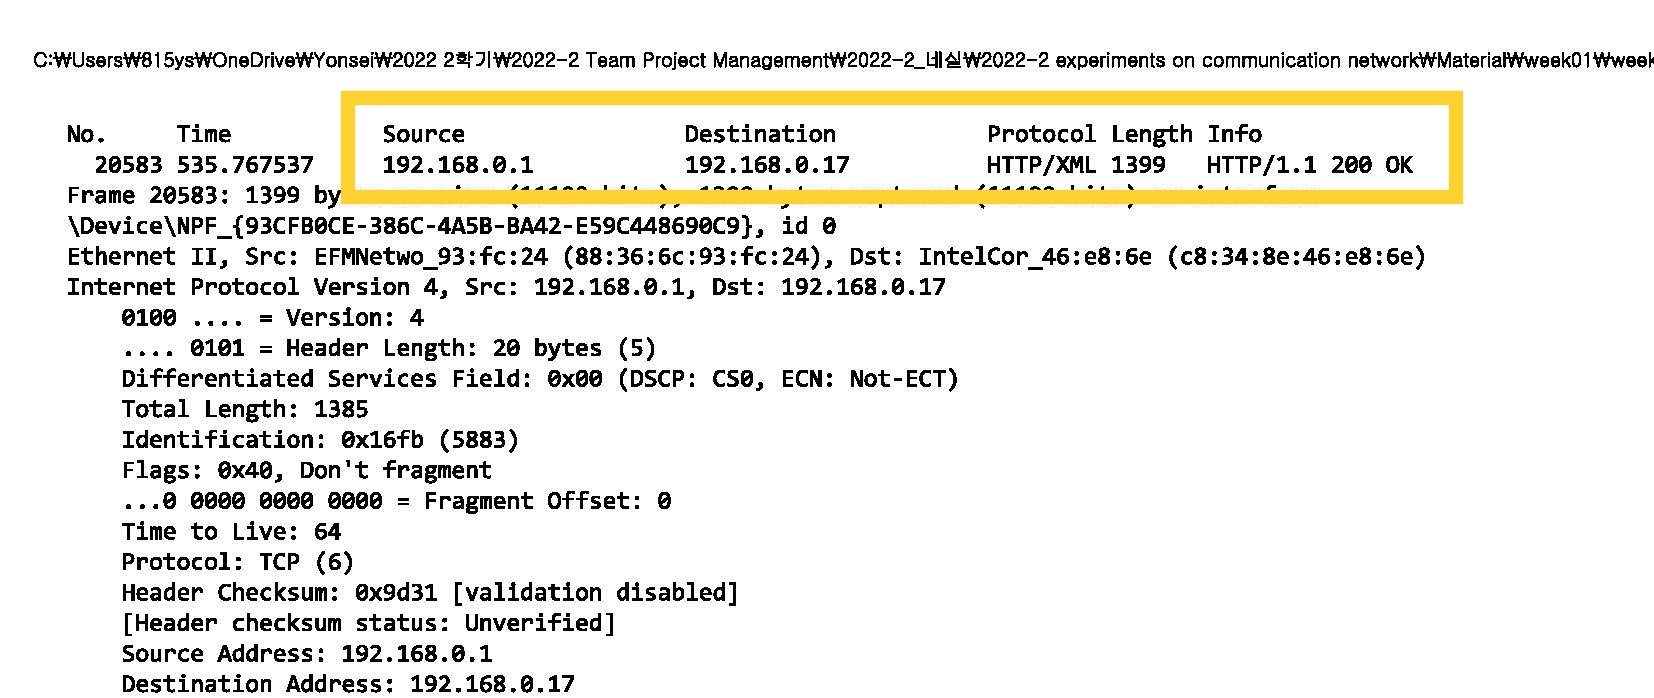
\includegraphics[width=.85\textwidth]{image/result_week01/Q1-3.jpg}
        		\caption{\footnotesize Problem 1-3's screenshot : Packet-HTTP/1.1 200 OK}
        		\vspace{-10pt}
            \end{figure}
        \item Print the two HTTP messages (GET and OK) referred to in question 2 above. 
        To do so, select Print from the Wireshark File command menu, and select the “Selected Packet Only” 
        and “Print as displayed” radial buttons, and then click OK.\\[0.2mm]
            \soln 
            \vspace{-4mm}  
            \begin{figure}[!h]\centering
            \hspace{15mm} 
        		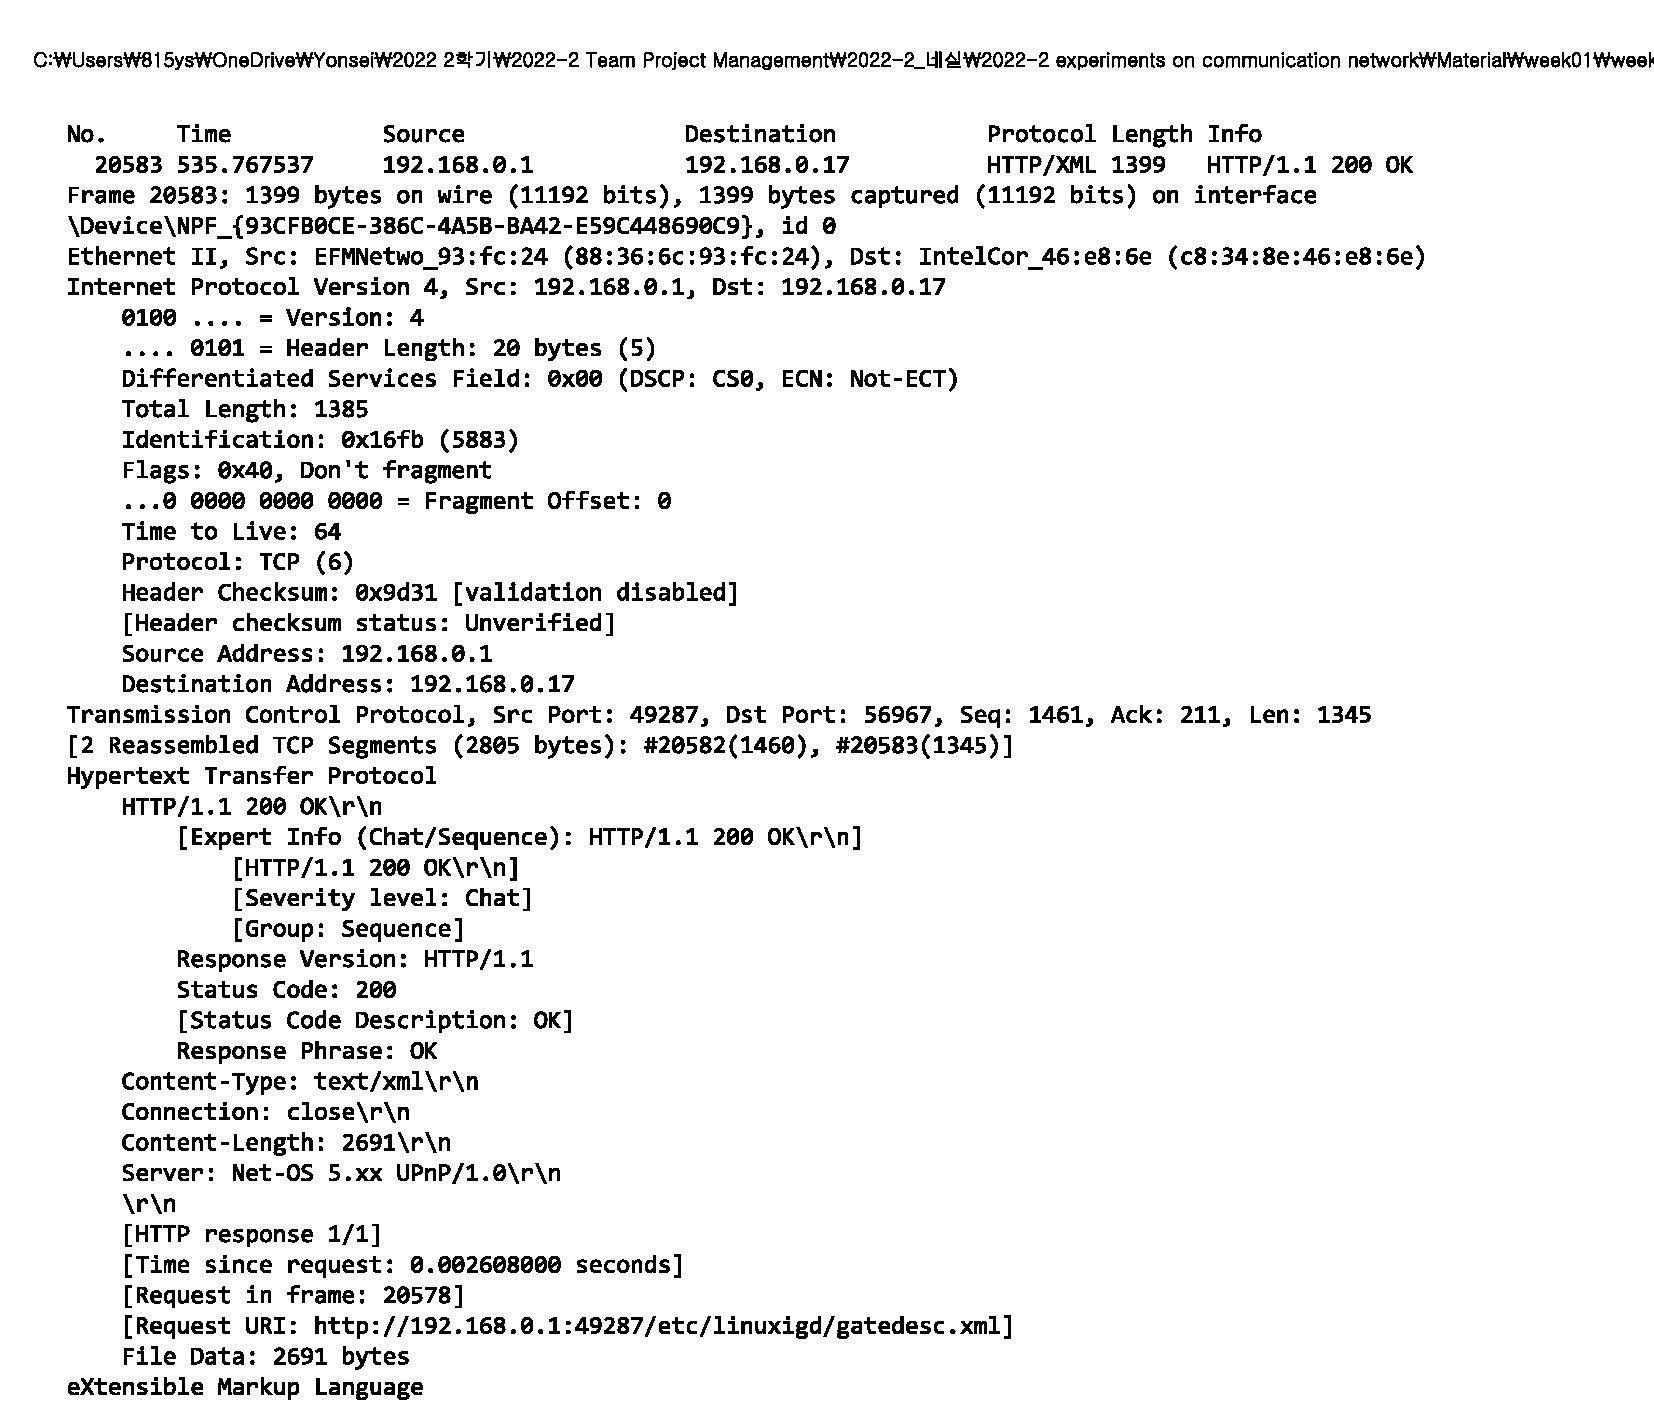
\includegraphics[width=.85\textwidth]{image/result_week01/Q1-4.jpg}
        		\caption{\footnotesize Problem 1-4's screenshot : Packet-HTTP/1.1 200 OK}
        		\vspace{-10pt}
            \end{figure}
    \end{enumerate}
\newpage